\chapter{Execute Stage}

\section{ALU: Arithmetic Logic Unit}
\subsection{Adder}
\subsection{Multiplier}
\subsection{Logic Operands}
The basic and most simple implementation of a logic unit is based on single logic gates on $N$ bits whose outputs are muxed, in order to generate the correct output. The problem with this solution is that the number of input signals to the multiplexer is extremely high; this implementation does not only suffer from the point of view of the delay but, since each logic function is implemented with a specific gate, the total area is huge.\newline\newline
In order to overcome the problems highlighted before, a more compact implementation has been chosen: the T2 logic unit.

This logic unit allows to perform AND, NAND, OR, NOR, XOR and XNOR using only 5 NAND gates, on two levels, and 4 selection signals. The schematic is the one in figure \ref{fig:log_unit}.

\begin{figure}
	\centering
	\tikzstyle{branch}=[fill,shape=circle,minimum size=3pt,inner sep=0pt]
	\begin{tikzpicture}[label distance=2mm]
		\draw (0.92,-0.40) -- (1.09,-0.56);
		\draw (1.92,-0.40) -- (2.09,-0.56);
		% nodes
		\node (y1) at (1,0) {$R_1$};
		\node (y2) at (2,0) {$R_2$};
		\node[not gate US, draw, rotate=-90] at ($(y1)+(0.5,-1.5)$) (noty1) {};
		\node[not gate US, draw, rotate=-90] at ($(y2)+(0.5,-1.5)$) (noty2) {};
		
		% draw nodes to NOT
		\foreach \i in {1,2} {
			\path (y\i) -- coordinate (punt\i) (y\i |- noty\i.input);
			\draw (punt\i) node[branch] {} -| (noty\i.input);
		}
	
		\node (x1) at (0,-2.33) {$S_0$};
		\node (x2) at (0,-3.33) {$S_1$};
		\node (x3) at (0,-4.33) {$S_2$};
		\node (x4) at (0,-5.33) {$S_3$};
		
		\node[nand gate US, draw, logic gate inputs=nnn] at ($(y2)+(2,-2.5)$) (And1) {};
		\node[nand gate US, draw, logic gate inputs=nnn] at ($(And1)+(0,-1)$) (And2) {};
		\node[nand gate US, draw, logic gate inputs=nnn] at ($(And2)+(0,-1)$) (And3) {};
		\node[nand gate US, draw, logic gate inputs=nnn] at ($(And3)+(0,-1)$) (And4) {};
		\node[nand gate US, draw, logic gate inputs=nnnn, anchor=input 1] at ($(And1.output -| And2.output)+(2,-1.25)$) (Or1) {};
		

		% connect x_i to AND_i
		\foreach \i in {1,2,3,4} {
			\draw (x\i) -- (And\i.input 1);
		}
		
		% y1

		\draw (noty1 |- And1.input 2) node[branch] {} -- (And1.input 2);
		\draw (noty1 |- And2.input 2) node[branch] {} -- (And2.input 2);
		\draw (y1 |- And3.input 2) node[branch] {} -- (And3.input 2);
		\draw (y1) |- (And4.input 2);
		\draw (noty1) |- (And2.input 2);
		
		\draw (noty2 |- And1.input 3) node[branch] {} -- (And1.input 3);
		\draw (y2 |- And2.input 3) node[branch] {} -- (And2.input 3);
		\draw (noty2 |- And3.input 3) node[branch] {} -- (And3.input 3);
		\draw (y2) |- (And4.input 3);
		\draw (noty2) |- (And3.input 3);
		

		% AND
		\draw (And1.output) -- ([xshift=0.8cm]And1.output) |- (Or1.input 1);
		\draw (And2.output) -- ([xshift=0.6cm]And2.output) |- (Or1.input 2);
		\draw (And3.output) -- ([xshift=0.6cm]And3.output) |- (Or1.input 3);
		\draw (And4.output) -- ([xshift=0.8cm]And4.output) |- (Or1.input 4);
	
		
		% OR
		\draw (Or1.output) -- ([xshift=0.5cm]Or1.output) node[above] {$out$};
		
	\end{tikzpicture}  
	\caption{Logic unit}
	\label{fig:log_unit}
	\end{figure}

	In order to compute one of the logical instructions, the select signals are properly activated as follow:
	
	\[
	\begin{vmatrix}
		S_0 & S_1 & S_2 & S_3 & \text{operation}\\
		0 & 0 & 0 & 1 & AND \\
		1 & 1 & 1 & 0 & NAND \\
		0 & 1 & 1 & 1 & OR \\
		1 & 0 & 0 & 0 & NOR \\
		0 & 1 & 1 & 0 & XOR \\
		1 & 0 & 0 & 1 & NXOR \\
	\end{vmatrix}
	\]
	
	
	For example, in order to generate the AND logical operation, we have to select $S_3 = 1$, so that $out = R_1 \cdot R_2$; on the other hand, if we need NAND $S_0 = S_1 = S_2 = 1$ and $S_3 = 0$, so that $out = \overline{R_1} \cdot \overline{R_2} + \overline{R_1} \cdot R_2 + R_1 \cdot \overline{R_2} = \overline{R_1} \cdot \overline{R_2}$ that using the De Morgan law $out = \overline{R_1 \cdot R_2}$.
	This allows to obtain the best performances also because all paths work in parallel, compacting the area and the delay.

\subsection{Shifting}
The implemented shifter allows to perform shift right, logical/arithmetical shift left and left/right rotate using the full operand \texttt{A} on 32 bits and 6 bits from the second one \texttt{B} and three \textit{control signals}.
Differently from the T2 version, it uses and addition signal in order to be able to manage also the rotate instruction. Our implementation takes three inputs:
\begin{itemize}
	\itemsep0sp
	\item \texttt{A}: the operand to be shifted/rotated;
	\item \texttt{B}: only the 5 LSB [4,3,2,1,0] are used to select first the mask to be used and then the starting point from that mask;
	\item \texttt{SEL}: it encodes the operation type; the second bit is used to select among arithmetic and logic, the third bit is used to select the direction of the shift/rotate (left/right) and the first one is used only if the operation is a rotate. This is the encoding:
	\begin{center}
		\begin{tabular}{c|l}
			\texttt{SEL} & \textbf{Operation}\\
			\hline
			000 & Shift logic right \\
			001 & Shift logic left \\
			010 & Shift arith right \\
			011 & Shift arith left \\
			100 & Rotate right \\
			101 & Shift right \\
		\end{tabular}
	\end{center}
\end{itemize}

\begin{figure}[ht]
	\centering
	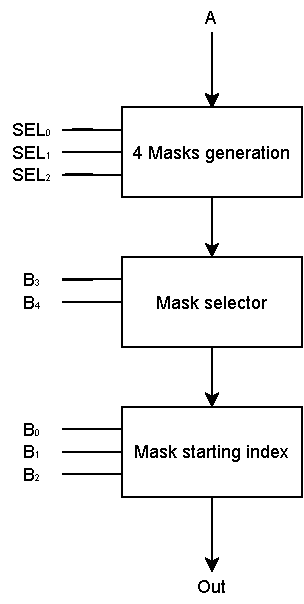
\includegraphics[width=0.2\textwidth]{chapters/5_ExecuteStage/images/Shifter.pdf}
	\caption{Blocks of the Shifter/Rotate Unit}
	\label{fig:shifter}
\end{figure}

 The unit perform the requested operation in three stages, sketched in figure \ref{fig:shifter}:
\begin{enumerate}
	\item The first consist in preparing 4 possible ``masks", each already shifted of {0, 8, 16, 32} left
	or right depending on the configuration. This allows to shift for all 32 bits. Basically it copies
	the input \texttt{A} into the 4 masks that will be used by the next stage. Being in 32 bits, the generated masks are in $32+8=40$ bits. The only different between this implementation and the T2 one, is that, in case of rotate, the additional 8 bits of the masks are filled with the corresponding 8 bits that are going ``out" during the rotation.
	
	\item The second level perform a coarse grain shift, that is basically consist on selecting one mask
	among the 4 possible masks generated in the previous stage. This selection is done by using the bits {4, 3} of \texttt{B}.
	\item The third level, using the bits {2, 1, 0} of \texttt{B} and the selected mask, preform a fine grain refinement. The 3 bits allows to select the starting index from the mask, in fact it allows to select among 8 positions.
\end{enumerate}



\begin{figure}[H] 
	\label{ fig7} 
	\begin{minipage}[b]{0.5\linewidth}
		\centering
		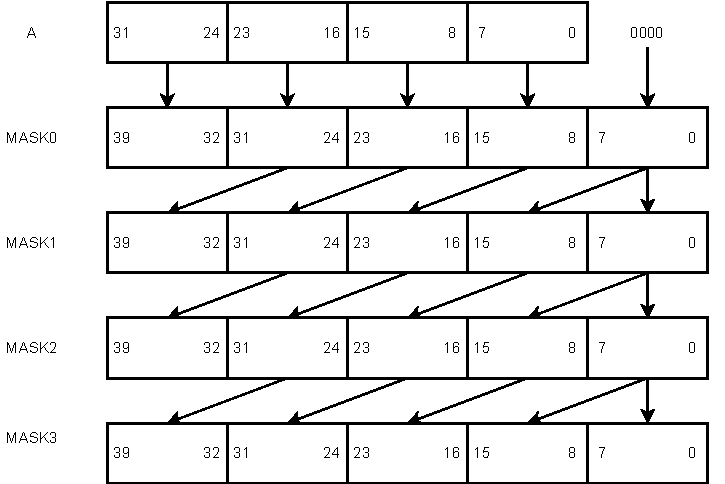
\includegraphics[width=.78\linewidth]{chapters/5_ExecuteStage/images/left_shift.pdf} 
		\caption{Masks for left shift} 
		\vspace{4ex}
	\end{minipage}%%
	\begin{minipage}[b]{0.5\linewidth}
		\centering
		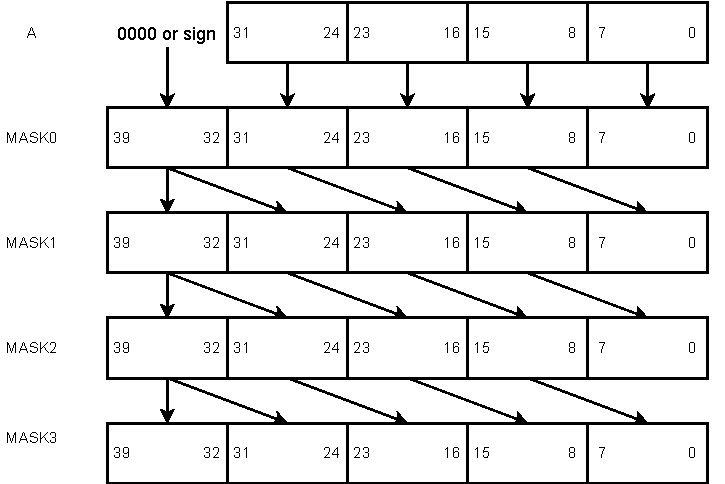
\includegraphics[width=.78\linewidth]{chapters/5_ExecuteStage/images/right_shift.pdf}
		\caption{Masks for right shift} 
		\vspace{4ex}
	\end{minipage} 
	\begin{minipage}[b]{0.5\linewidth}
		\centering
		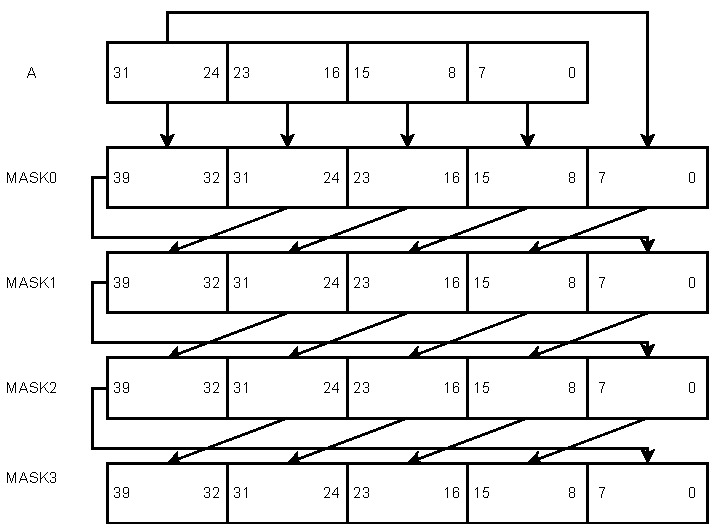
\includegraphics[width=.78\linewidth]{chapters/5_ExecuteStage/images/left_rotate.pdf} 
		\caption{Masks for left rotate} 
		\vspace{4ex}
	\end{minipage}%% 
	\begin{minipage}[b]{0.5\linewidth}
		\centering
		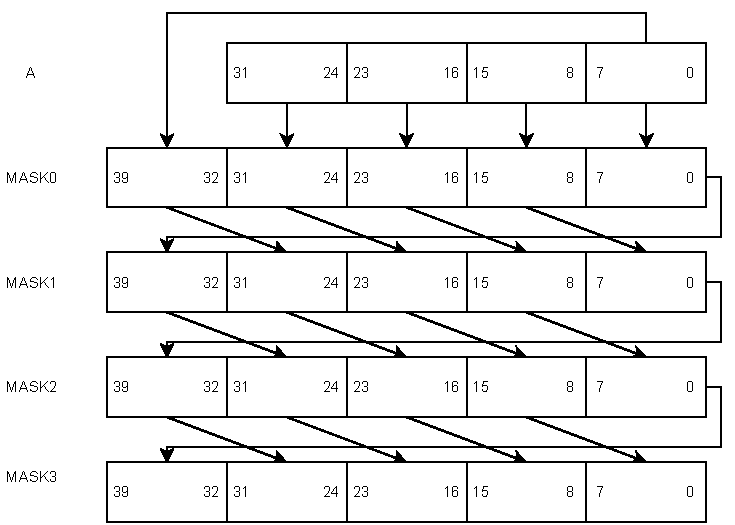
\includegraphics[width=.78\linewidth]{chapters/5_ExecuteStage/images/right_rotate.pdf} 
		\caption{Masks for right rotate} 
		\vspace{4ex}
	\end{minipage} 
\end{figure}
\begin{mybox}
	\textbf{Examples}
	\newline
	For example, if we need to perform a left left of 9 bits \texttt{A}, where \texttt{A=18}, the corresponding \texttt{B} value will be 1001; this means that the second masks will be taken and the output result will from the bit at position $40-1=39$ to the one at $39-32=7$ included.
	\begin{center}
		MASK 2: 0$\underbrace{\textbf{0000000 00000000 00000000 00010010 0}}_{\text{shifted \texttt{A}}}$0000000
	\end{center}
	
	On the other hand, if we need to perform a right shift the masks are generated in the opposite way, so the zeros are put in the MSB of the mask, shifted by 0, 8 ... positions. In this case we need also to distinguish between the an arithmetic and a logic shift; in the first case, instead of filling the ``empty" bits with zero, the operand sign is used. For example, if we want to shift \texttt{A=-18} of \texttt{B=3} bits, the first mask is used: 
	\begin{center}
		MASK 1: 11111$\underbrace{\textbf{111 11111111 11111111 11111111 11101}}_{\text{shifted \texttt{A}}}$110
	\end{center}
	
	In the last case, let's suppose to rotate right \texttt{A=1255} (=10011100111) by 5 position:
	\begin{center}
		MASK 1: 11$\underbrace{\textbf{100111 00000000 00000000 0000100 111}}_{\text{rotated \texttt{A}}}$00111
	\end{center}
	As you can see, in case of MASK 1 for the right rotation, the 8 LSB of \texttt{A} are copied into the 8 MSB of the mask.
\end{mybox}
	

\section{Set-Like Operations unit}
- setcmp